% ------------------------------------------------------------------------------
% TYPO3 Version 10 LTS - What's New (English Version)
%
% @author	Michael Schams <schams.net>
% @license	Creative Commons BY-NC-SA 3.0
% @link		https://typo3.org/help/documentation/whats-new/
% @language	English
% ------------------------------------------------------------------------------

\section{Formulierenraamwerk}
\begin{frame}[fragile]
	\frametitle{Formulierenraamwerk}

	\begin{center}\huge{\color{typo3darkgrey}\textbf{Formulierenraamwerk}}\end{center}
	\begin{center}\large{\textit{Eenvoudiger aanmaken en beheren van formulieren}}\end{center}

\end{frame}

% ------------------------------------------------------------------------------
% Feature | 79445 | Add Multistep Wizard

\begin{frame}[fragile]
	\frametitle{Formulierenraamwerk}
	\framesubtitle{Meerstapsassistent}

	\begin{itemize}
		\item Er is een nieuwe JavaScript module \texttt{MultiStepWizard},
			met de volgende functies:

			\begin{itemize}
				\item Navigatie naar vorige stappen.
				\item Stappen ondersteunen beschrijvende labels zoals "Begin" of "Einde", in plaats van nummers zoals "Stap x van y".
				\item Geoptimaliseerde configuratiestructuur.
			\end{itemize}

		\item Zie \href{https://docs.typo3.org/c/typo3/cms-core/master/en-us/Changelog/10.2/Feature-79445-AddMultistepWizard.html}{Overzicht wijzigingen}
			voor voorbeelden van JavaScript code.

		\item Deze functies verbeteren de gebruikerservaring enorm: backend-gebruikers hebben een verbeterde assistent voor het maken van formulieren.

	\end{itemize}

\end{frame}

% ------------------------------------------------------------------------------
% Feature | 84757 | Double click in structure tree changes label

\begin{frame}[fragile]
	\frametitle{Backend Gebruikersinterface}
	\framesubtitle{Titels bewerken}

	Labels van formulierelementen kunnen bewerkt worden door te dubbelklikken op de titel in de boom.

	\begin{figure}
		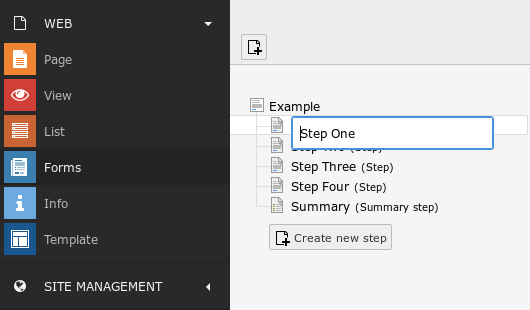
\includegraphics[width=0.5\linewidth]{FormFramework/84757-DoubleClickToChangeLabel.png}
	\end{figure}

\end{frame}

% ------------------------------------------------------------------------------
% Important | 84221 | Restructuring of form setup

\begin{frame}[fragile]
	\frametitle{Formulierenraamwerk}
	\framesubtitle{Formulierdefinitie}

	\begin{itemize}
		\item Voorheen werden drie bestanden gebruikt: \texttt{BaseSetup.yaml}, \texttt{FormEditorSetup.yaml}, en \texttt{FormEngineSetup.yaml}.
		\item Deze zijn samengevoegd in een enkel bestand: \texttt{FormSetup.yaml}.
		\item Dit bestand bevat de basisopzet en imports van configuratie voor validators, formulierelementen en finishers.
		\item Alle voorheen gebruikte overervingen en mixins zijn opgelost waardoor het eenvoudiger wordt om de configuratie te begrijpen.
	\end{itemize}

\end{frame}

% ------------------------------------------------------------------------------
% Breaking | 87009 | Use multiple translation files by default in EXT:form

\begin{frame}[fragile]
	\frametitle{Formulierenraamwerk}
	\framesubtitle{Vertalingn}

	% decrease font size for code listing
	\lstset{basicstyle=\tiny\ttfamily}

	\begin{itemize}
		\item De volgende optie is hernoemd:\newline
			\small\texttt{translationFile} \textrightarrow\hspace{0.1cm}\texttt{translationFiles}\normalsize
		\item De standaard taalbestanden zijn nu geregistreerd in index 10:

			\begin{itemize}
				\item \texttt{EXT:form/Resources/Private/Language/locallang.xlf}
				\item \texttt{EXT:form/Resources/Private/Language/Database.xlf}
			\end{itemize}

		\item Maatwerk YAML configuratiebestanden moeten bijgewerkt worden.
\begin{lstlisting}
OUD:
translationFile: path/to/locallang.xlf

NIEUW:
translationFiles:
  20: path/to/locallang.xlf
\end{lstlisting}

	\end{itemize}

\end{frame}

% ------------------------------------------------------------------------------
% Feature | 84203 | Unify form setup YAML loading

\begin{frame}[fragile]
	\frametitle{Formulierenraamwerk}
	\framesubtitle{YAML-bestanden}

	\begin{itemize}
		\item YAML-bestanden gebruiken nu de YAML-lader van de TYPO3 core.
		\item Dit biedt functies als:

			\begin{itemize}
				\item Andere YAML-bestanden importeren via \texttt{imports} aanwijzing.
				\item Vervanging van \texttt{\%placeholders\%}.
			\end{itemize}

	\end{itemize}

\end{frame}

% ------------------------------------------------------------------------------
% Feature | 90052 | Form YAML configuration available in configuration module

\begin{frame}[fragile]
	\frametitle{Formulierenraamwerk}
	\framesubtitle{YAML configuratie}

	\begin{columns}[T]
		\begin{column}{.04\textwidth}
		\end{column}
		\begin{column}{.38\textwidth}

			Als de systeemextensie \texttt{EXT:form} is geïnstalleerd kan de YAML-configuratie
			getoond worden onder \textbf{SYSTEEM} $\rightarrow$ \textbf{Configuratie}.

			\vspace{0.2cm}

			Admins moeten natuurlijk ook \texttt{EXT:lowlevel} geïnstalleerd hebben.

		\end{column}
		\begin{column}{.58\textwidth}
			\vspace{-0.3cm}
			\begin{figure}
				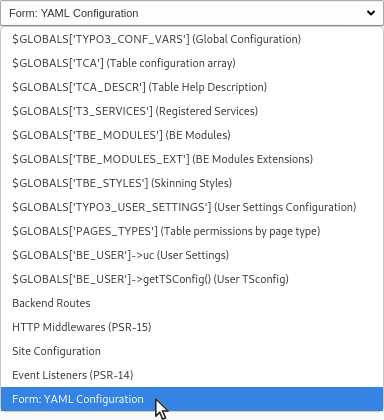
\includegraphics[width=0.70\linewidth]{FormFramework/90052-AddYamlConfigurationToConfigurationModule.png}
			\end{figure}
		\end{column}
	\end{columns}

\end{frame}

% ------------------------------------------------------------------------------
% Feature | 89747 | Custom tables with record browser in forms

\begin{frame}[fragile]
	\frametitle{Formulierenraamwerk}
	\framesubtitle{Bladeren door records}

	% decrease font size for code listing
	\lstset{basicstyle=\tiny\ttfamily}

	\begin{itemize}
		\item Het bladeren door records kan geconfigureerd worden om gebruikerstabellen te gebruiken:
\begin{lstlisting}
TYPO3:
  CMS:
    Form:
      prototypes:
        standard:
          formElementsDefinition:
            MyCustomElement:
              formEditor:
                editors:
                  # ...
                  300:
                    identifier: myRecord
                    # ...
                    browsableType: tx_myext_mytable
                    propertyPath: properties.myRecordUid
                    # ...
\end{lstlisting}

	\end{itemize}

\end{frame}

% ------------------------------------------------------------------------------
% Feature | 89746 | Custom icon for record browser button in forms

\begin{frame}[fragile]
	\frametitle{Formulierenraamwerk}
	\framesubtitle{Bladeren door records}

	% decrease font size for code listing
	\lstset{basicstyle=\tiny\ttfamily}

	\begin{itemize}
		\item Het icoon op de knop voor het bladeren door records is instelbaar:
\begin{lstlisting}
TYPO3:
  CMS:
    Form:
      prototypes:
        standard:
          formElementsDefinition:
            MyCustomElement:
              formEditor:
                editors:
                  # ...
                  300:
                    identifier: contentElement
                    # ...
                    browsableType: tt_content
                    iconIdentifier: mimetypes-x-content-text
                    propertyPath: properties.contentElementUid
                    # ...
\end{lstlisting}

	\end{itemize}

\end{frame}

% ------------------------------------------------------------------------------
% Feature | 84713 | Access single values in form templates

\begin{frame}[fragile]
	\frametitle{Formulierenraamwerk}
	\framesubtitle{Bladeren door records}

	% decrease font size for code listing
	\lstset{basicstyle=\tiny\ttfamily}

	\begin{itemize}
		\item Een nieuwe \textit{RenderFormValue-ViewHelper} zorgt voor toegang tot losse formulierwaardes in sjablonen voor integrators/developers:
\begin{lstlisting}
<p>
  Het volgende bericht was verstuurd door
  <formvh:renderFormValue renderable="{page.rootForm.elements.name}" as="formValue">
    {formValue.processedValue}
  </formvh:renderFormValue>:
</p>

<blockquote>
  <formvh:renderFormValue renderable="{page.rootForm.elements.message}" as="formValue">
    {formValue.processedValue}
  </formvh:renderFormValue>
</blockquote>
\end{lstlisting}

	\end{itemize}

\end{frame}

% ------------------------------------------------------------------------------
% Feature | 82706 | Render fieldset labels in form templates

\begin{frame}[fragile]
	\frametitle{Formulierenraamwerk}
	\framesubtitle{Labels set velden}

	\begin{itemize}
		\item Het sectie-element \texttt{Fieldset} is nu toegankelijk in sjablonen.
		\item Standaard heeft dit invloed op zowel het \textbf{SummaryPage} formulierelement als de \textbf{EmailToReceiver} en \textbf{EmailToSender} finishers.
		\item Voorbeeld toepassing:\newline
			\small
				Een formulier met verzend- en factuuradres. Beide secties kunnen een veld hebben met dezelfde naam, bijv. \texttt{straat}.
				Er kan nu onderscheid gemaakt worden tussen de velden door de labels van de Fieldset.
			\normalsize

	\end{itemize}

\end{frame}

% ------------------------------------------------------------------------------
% Deprecation | 88238 | Allowed MIME types of FileUpload and ImageUpload

\begin{frame}[fragile]
	\frametitle{Formulierenraamwerk}
	\framesubtitle{Bestanden uploaden}

	\begin{itemize}
		\item Voorgedefinieerde \texttt{allowedMimeTypes} van de volgende formulierelementen zijn als \textbf{verouderd} aangemerkt:

			\begin{itemize}
				\item \texttt{FileUpload}
				\item \texttt{ImageUpload}
			\end{itemize}

		\item Alle geldige MIME-types moeten nu expliciet opgesomd worden in de formulierdefinitie\newline
			\smaller
				(voorgedefinieerde MIME-types worden verwijderd in TYPO3 v11)
			\normalsize

	\end{itemize}

\end{frame}

% ------------------------------------------------------------------------------
% Deprecation | 89742 | Form mixins

\begin{frame}[fragile]
	\frametitle{Formulierenraamwerk}
	\framesubtitle{Formulier-mixins}

	\begin{itemize}
		\item Mixins zijn als \textbf{verouderd} aangemerkt en zouden niet meer gebruikt moeten worden.
		\item Dit geldt voor alle overervingen van \texttt{TYPO3.CMS.Form.mixins.*}.
		\item Opties voor migratie:

			\begin{itemize}
				\item Voeg de essenti\"ele delen van \texttt{TYPO3.CMS.Form.mixins.*} in, of
				\item verhuis ze naar maatwerk-mixins.
			\end{itemize}

	\end{itemize}

\end{frame}

% ------------------------------------------------------------------------------
% Feature | 80420 | Allow multiple recipients in email finisher

\begin{frame}[fragile]
	\frametitle{Formulierenraamwerk}
	\framesubtitle{Meerdere ontvangers}

	\begin{itemize}
		\item Mails kunnen door de \textit{EmailFinisher} verstuurd worden aan meerdere ontvangers.

		\item De volgende nieuwe opties zijn ge\"{\i}ntroduceerd:

			\begin{itemize}
				\item \texttt{recipients} (To)
				\item \texttt{replyToRecipients} (Reply-To)
				\item \texttt{carbonCopyRecipients} (CC)
				\item \texttt{blindCarbonCopyRecipients} (BCC)
			\end{itemize}

	\end{itemize}

\end{frame}

% ------------------------------------------------------------------------------
% Feature | 80420 | Allow multiple recipients in email finisher

\begin{frame}[fragile]
\frametitle{Formulierenraamwerk}
\framesubtitle{Meerdere ontvangers}

	% decrease font size for code listing
	\lstset{basicstyle=\tiny\ttfamily}

	\begin{itemize}
		\item Deze wijziging vergt het handmatig aanpassen van enkele waarden naar lijsten.

		\smaller\textbf{Oude} Finisher configuratie:\normalsize
\begin{lstlisting}
finishers:
  -
    identifier: EmailToReceiver
    options:
      recipientAddress: user@example.com
      recipientName: 'Voornaam Achternaam'
\end{lstlisting}

		\smaller\textbf{Nieuwe} Finisher configuratie:\normalsize
\begin{lstlisting}
finishers:
  -
    identifier: EmailToReceiver
    options:
      recipients:
        user@example.com: 'Voornaam Achternaam'
\end{lstlisting}

		\item Zie \href{https://docs.typo3.org/c/typo3/cms-core/10.0/en-us/Changelog/master/Deprecation-80420-EmailFinisherSingleAddressOptions.html}{change log}
			voor meer migratievoorbeelden.

	\end{itemize}

\end{frame}

% ------------------------------------------------------------------------------
% Deprecation | 87200 | EmailFinisher format option
% Deprecation | 87200 | EmailFinisher FORMAT_* constants

\begin{frame}[fragile]
	\frametitle{Formulierenraamwerk}
	\framesubtitle{Platte tekst/HTML}

	\begin{itemize}
		\item Mails verstuurd door de \textit{EmailFinisher} kunnen zowel een HTML en/of tekstdeel hebben.

		\item Tegelijkertijd is de optie \texttt{format} aangemerkt als verouderd en zal verwijderd worden in TYPO3 v11.

		\item Bestaande waarden zullen automatisch gemigreerd worden:

			\begin{itemize}\smaller
				\item \texttt{format:html} \tabto{3cm}\textrightarrow\hspace{0.1cm}\texttt{addHtmlPart:\textbf{true}}
				\item \texttt{format:plaintext} \tabto{3cm}\textrightarrow\hspace{0.1cm}\texttt{addHtmlPart:\textbf{false}}
				\item een ontbrekend "\texttt{format}" \tabto{3cm}\textrightarrow\hspace{0.1cm}\texttt{addHtmlPart:\textbf{true}}
			\end{itemize}\normalsize

		\item Ontwikkelaars moeten letten op de volgende twee constanten die als verouderd gemarkeerd zijn:

			\begin{itemize}\smaller
				\item \texttt{EmailFinisher::FORMAT\_PLAINTEXT}
				\item \texttt{EmailFinisher::FORMAT\_HTML}
			\end{itemize}\normalsize

	\end{itemize}

\end{frame}

% ------------------------------------------------------------------------------
% Feature | 87798 | Provide a way to sort form lists in ext:form

\begin{frame}[fragile]
	\frametitle{Gedetailleerde wijzigingen}
	\framesubtitle{Sorteren van formulieren}

	% decrease font size for code listing
	\lstset{basicstyle=\tiny\ttfamily}

	\begin{itemize}
		\item Formulieren kunnen nu zowel oplopend als aflopend worden gesorteerd.
		\item Twee nieuwe instellingen zijn ge\"{\i}ntroduceerd: \texttt{sortByKeys} en \texttt{sortAscending}.
		\item Formulieren worden in de basis gesorteerd op naam en bestands-UID (oplopend).
		\item Om de sortering te wijzigen moet de volgende configuratie worden toegevoegd in de YAML configuratiebestanden:
\begin{lstlisting}
TYPO3:
  CMS:
    Form:
      persistenceManager:
        sortByKeys: ['name', 'fileUid']
        sortAscending: true
\end{lstlisting}

	\end{itemize}

\end{frame}

% ------------------------------------------------------------------------------
